\begin{frame}{Satellite Quantum Key Distribution (QKD)}
    \visible<1->{
        Quantum Key Distribution.
        % \begin{itemize}
        %     \item Cryptographic protocol involving components of quantum mechanics.
        %     \item Enables two parties to produce a shared random secret key known only to them.
        % \end{itemize}
    }
    
    \begin{overprint}
        \onslide<1>
        \begin{itemize}
            \item Cryptographic protocol involving components of quantum mechanics.
            \item Enables two parties to produce a shared random secret key known only to them.
        \end{itemize}
        \onslide<2->
        Satellite QKD: share random key between satellite and ground station.
        \visible<3->{
        
        A classical channel is used along to synchronise quantum channel~\sfcite{zhang2021timing,khader2018time}.
        \begin{figure}
            \centering
            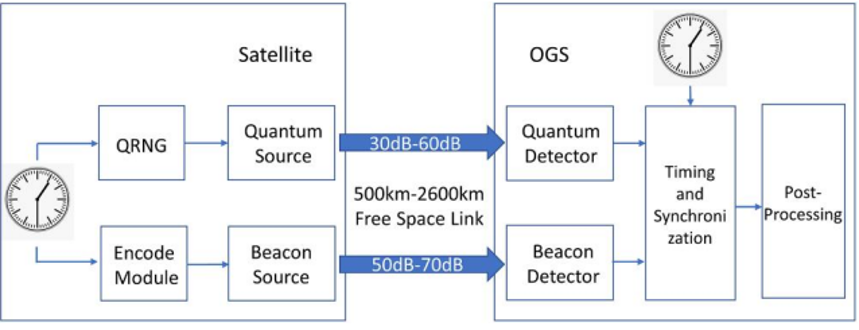
\includegraphics[scale=.3]{Images/Motivation/SatteliteQKD.png}
            \caption{High-level satellite Quantum Key Distribution schematic~\sfcite{zhang2021timing}.}
            \label{fig:satelliteQKD}
        \end{figure}
    }    
    \end{overprint}
    
    % \visible<2->{
    %     Satellite QKD: share random key between satellite and ground station
        
    % }
    
    % \visible<3->{
    %     A classical channel is used along to synchronise quantum channel~\sfcite{duan2021survey,khader2018time}.
    %     \begin{figure}
    %         \centering
    %         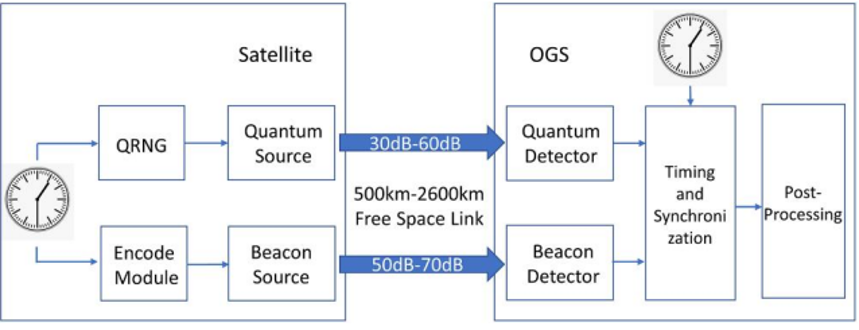
\includegraphics[scale=.3]{Images/Motivation/SatteliteQKD.png}
    %         \caption{High-level satellite Quantum Key Distribution schematic.}
    %         \label{fig:satelliteQKD}
    %     \end{figure}
    % }
\end{frame}

% \begin{frame}{Satellite Quantum Key Distribution (QKD)}
%     Commercial QKD: deployed over optical fibre.
%     \begin{overprint}
%         \onslide<1>
%         But: $$\mathrm{range}< 1000 \mathrm{km}$$
%         \onslide<2>
%         But: $$\mathrm{range}< 1000 \mathrm{km}$$
%         $\rightarrow$ Satellite QKD: alternative method to establishing intercontinental secure communication links.
        
%         \onslide<3> 
%         But: $$\mathrm{range}< 1000 \mathrm{km}$$
%         $\rightarrow$ Satellite QKD: alternative method to establishing intercontinental secure communication links.
        
%         Challenges:
%         \begin{itemize}
%             \item High channel losses.
%             \item Rapid relative motion between the transmitter and receiver.
%         \end{itemize}
%         \onslide<4-> 
%         % \visible<4->{
%         $\rightarrow$ Satellite QKD: alternative method to establishing intercontinental secure communication links.
        
%         $\rightarrow$ A classical channel is used along to synchronise quantum channel~\sfcite{duan2021survey,khader2018time}.
%         \begin{figure}
%             \centering
%             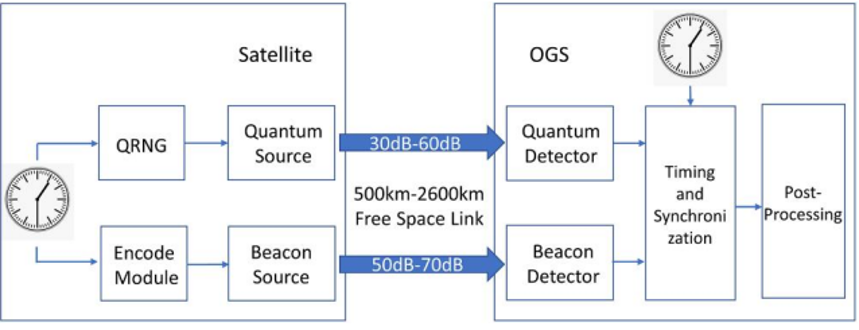
\includegraphics[scale=.3]{Images/Motivation/SatteliteQKD.png}
%             \caption{High-level satellite Quantum Key Distribution schematic.}
%             \label{fig:satelliteQKD}
%         \end{figure}
%         % }
%     \end{overprint}
    
%     % \visible<3->{
%     %     $\Rightarrow$ A classical channel is used along to synchronise quantum channel~\sfcite{duan2021survey,khader2018time}.
%     %     \begin{figure}
%     %         \centering
%     %         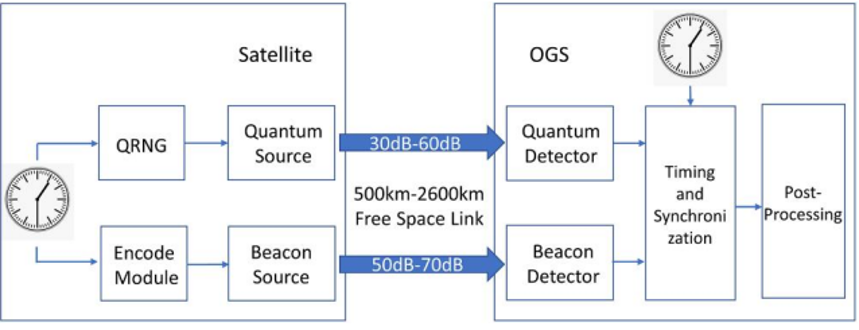
\includegraphics[scale=.3]{Images/Motivation/SatteliteQKD.png}
%     %         \caption{High-level satellite Quantum Key Distribution schematic.}
%     %         \label{fig:satelliteQKD}
%     %     \end{figure}
%     % }
% \end{frame}


\begin{frame}{Related Work}
    \citeauthor{zhang2021timing}\sfcite{zhang2021timing}: de Bruijn based timing-synchronization system (dBTS).
    \begin{overprint}
        \onslide<2-4> 
            \begin{columns}
            \visible<2->{
                \begin{column}{.37\textwidth}
                    \begin{centering}
                        \fcolorbox{red}{white}{Encode}
                        \begin{figure}
                            % \centering
                            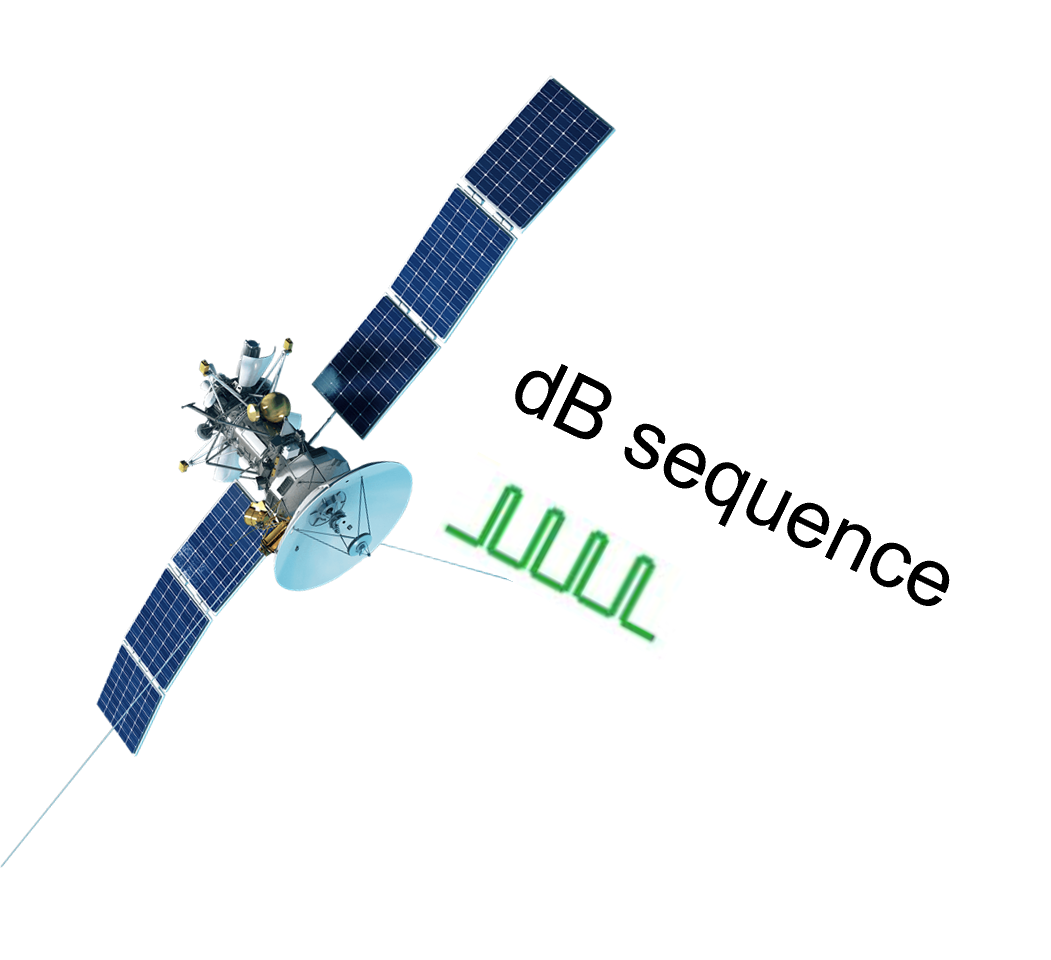
\includegraphics[width=0.6\textwidth]{Images/Motivation/SatelliteEncode.png}
                            % \caption{Caption}
                            % \label{fig:my_label}
                        \end{figure}
                    \end{centering}
                    \begin{itemize}
                        \item Linear feedback shift register (LFSR): generate an order $k$ de Bruijn sequence.
                    \end{itemize}
                \end{column}
                \vrule{}
            }
            \visible<3->{
                \begin{column}{.26\textwidth}
                    \begin{centering}
                        \fcolorbox{red}{white}{Noisy channel}
                        \begin{figure}
                            % \centering
                            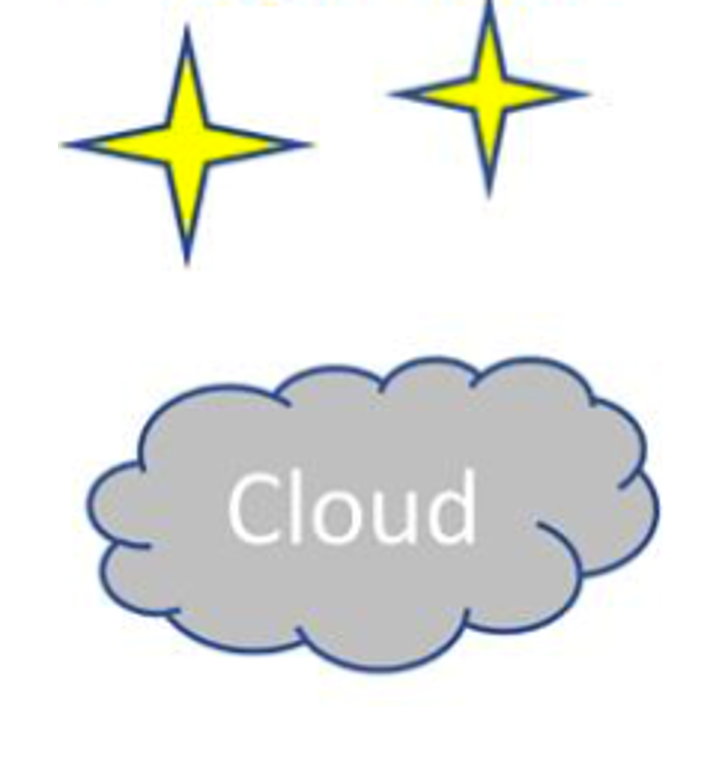
\includegraphics[width=0.6\textwidth]{Images/Motivation/Cloud.png}
                            % \caption{Caption}
                            % \label{fig:my_label}
                        \end{figure}
                    \end{centering}
                \end{column}
                \vrule{}
            }
            \visible<4->{
                \begin{column}{.37\textwidth}
                    \begin{centering}
                        \fcolorbox{red}{white}{Decode}
                        \begin{figure}
                            % \centering
                            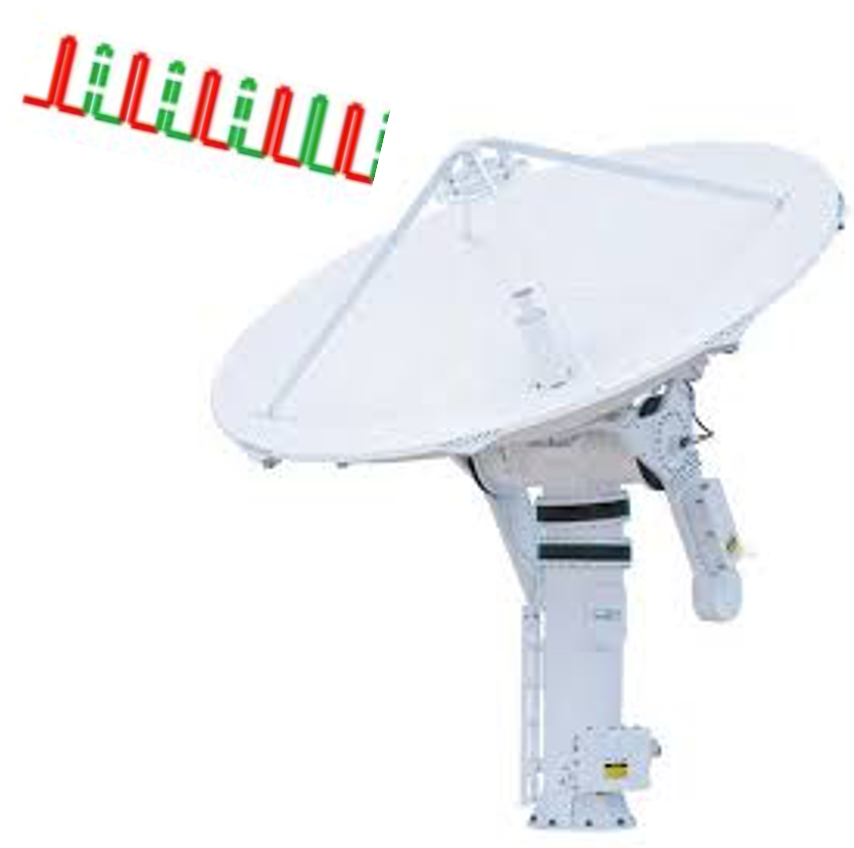
\includegraphics[width=0.5\textwidth]{Images/Motivation/GSDecode.png}
                            % \caption{Caption}
                            % \label{fig:my_label}
                        \end{figure}
                    \end{centering}
                    \begin{itemize}
                        \item Look-up table: locate the position of a length $k$ subsequence in the whole sequence.
                    \end{itemize}
                \end{column}
            }
            \end{columns}
        \onslide<5->
            \visible<5->{
                \begin{block}{Transmit a modulated sequence}
                    \begin{itemize}
                        \item {\color{red}Constraint}: avoid long period of no pulse .
                        \item {\color{red}Requirement}: positioning sequence.
                        \item {\color{red}Method}: de Bruijn sequence, pulse modulation: $1\rightarrow\mathrm{on-on},\ 0\rightarrow\mathrm{on-off}$, called Hybrid de Bruijn (HdB) sequence.
                    \end{itemize}
                \end{block}
            }
            \visible<6->{
                \begin{alertblock}{Drawback}
                    \begin{itemize}
                        \item $\mathrm{Rate}=0.5$.
                        \item Encode: LFSR (prerequisite: suitable primitive polynomial).
                        \item Decode: use look-up table (exponential complexity).
                    \end{itemize}
                \end{alertblock}
            }
    \end{overprint}
    
\end{frame}

\begin{frame}{Contributions}
    \begin{block}{Propose a new combinatorial object RdB}
        \begin{itemize}
            \item Can be encoded and decoded efficiently.
            \item Can replace HdB sequence: higher rate and maximal asymptotic rate, more general and adaptive.
        \end{itemize}
    \end{block}
    \begin{block}{Determine the maximal length of RdB}
        \begin{itemize}
            \item Explicit formula.
        \end{itemize}
    \end{block}
    \begin{block}{Encoding and Decoding Algorithm}
        \begin{itemize}
            \item Encoder: Constant amortized time per symbol.
            \item Decoder: Sub-linear time with respect to the length of the sequence.
        \end{itemize}
    \end{block}
\end{frame} 

